When we first deployed ORES, we reached out to several different wiki communities and invited them to test the system for use in patrolling for vandalism.  In these announcements, we encouraged editors to install ScoredRevisions, the only tool that used ORES's edit quality models at the time.  ScoredRevisions both highlights edits that are likely to be damaging (as predicted by the model) and displays the likelihood of the prediction as a percentage.

Before long, our users began filing false-positive reports on wiki pages of their own design.  In this section, we describe three cases where our users independently developed these false-positive reporting pages and how they used them to understand ORES, the roles of automated quality control in their own spaces, and to communicate with us about ORES.

\subsection{Report mistakes (Wikidata)}
\begin{figure}[h]
  \centering
  \includegraphics[width=.45\textwidth]{figures/ORES_report_mistakes_table}
  \caption{A slice of the ORES report mistakes table in Wikidata.}
  \label{fig:ores_report_mistakes}
\end{figure}

When we first deployed prediction models for Wikidata---a free and open knowledge base that can be read and edited by both humans and machines\footnote{\url{https://wikidata.org}}---we were breaking new ground by building a damage detection classifier based on a structured data wiki\cite{sarabadani2017building}.  We created a page called ``Report mistakes'' and invited users to tell us about mistakes that the prediction model made on that page. We left the format and structure largely up to the users.

Within 20 minutes, we received our first report, from an editor who believed ORES was reporting edits that couldn't possibly be vandalism as potentially damaging.  As reports streamed in, we began to respond to them and make adjustments to the model building process to address data extraction bugs and to increase the signal so that the model differentiate damage from non-damaging edits.  After a month of reports and bug fixes, we decided to build a table to represent the progress that we made in iterations on the model against the reported false-positives (Figure~\ref{fig:ores_report_mistakes}).  Each row represents a mis-classified edit, and each column describes the progress we made in not detecting those edits as damaging in future iterations of the model.  Through this process, we learned how Wikidata editors understood and saw damage, as well as how our modeling and feature extraction process captured signals in ways that differed from Wikidata editors' understandings.  Because of this back-and-forth collaboration made possible through ORES's various features, we were able to publicly demonstrate improvements to this community.

\subsection{Patrolling/ORES (Italian Wikipedia)}
Italian Wikipedia was one of the first wikis where we deployed basic edit quality models.  Our local collaborator, who helped us develop the language specific features, User:Rotpunkt, created a page for ORES\footnote{\url{https://it.wikipedia.org/wiki/Progetto:Patrolling/ORES}} with a section for reporting false-positives (``falsi positivi'').  Within several hours, Rotpunkt and a few other editors noticed some trends in their false positive reports.  First, Rotpunkt noticed that there were several counter-vandalism edits that ORES was flagging as potentially damaging, so he made a section for collecting that specific type of mistake (``annullamenti di vandalismo'').  A few reports later, he added a section for ``corrections to the verb for \emph{have}'' (``correzioni verbo avere'').  Through this process, editors from Italian Wikipedia were effectively performing an inductive, grounded theory-esque exploration ORES errors, trying to identify themes and patterns in the errors that ORES was making.

Once there were several of these mistake-type sections and several reports within each section, Rotpunkt reached out to us to let us know what he had found.  He explained to us (via our IRC channel) that many of ORES's mistakes were understandable, but there were some general trends in mistakes around the Italian verb for \emph{have}: ``ha''.  We knew immediately what was likely to be the issue. A common type of vandalism in English and other languages is to add the word ``ha'' repeatedly to indicate laughing, and so a common feature in the damage model was ``informal words'' that are not blatantly offensive, but generally likely to not be constructive additions to encyclopedia articles.  However, the word ``ha'' in Italian translates to ``have'' and is perfectly acceptable in articles in that language.

Because of the work of Rotpunkt and his collaborators in Italian Wikipedia, we were able to recognize the source of this issue (a set of features intended to detect the use of \emph{informal language} in articles) and to remove ``ha'' from that list for Italian Wikipedia.  This is just one example of many issues we were able to address because of the grounded theory and thematic analysis performed by Italian Wikipedians.

\subsection{PatruBOT (Spanish Wikipedia)}
Soon after we released support for Spanish Wikipedia, a volunteer developer made a software bot to automatically revert damaging edits using ORES's predictions for the ``damaging'' model (PatruBOT).  This bot was not running for long before our discussion pages were bombarded with confused Spanish-speaking editors asking us questions about why ORES did not like their work.  We struggled to understand the origin of the complaints until someone reached out about PatruBOT and its activities.

When we examined the case, we found it was one of tradeoffs between precision/recall and false positives/negatives -- a common issue with machine learning applications. We concluded that PatruBOT's thresholds for reverting were too sensitive for many in the Spanish Wikipedia community, meaning it was likely reverting edits that the model did not have enough confidence about. ORES reports a classification and a probability score, but it is up to the developers to decide if, for example, the bot will only auto-revert edits classified as damage with a .90, .95, .99, or higher likelihood estimate. A higher threshold will minimize the chance a good edit will be mistakenly auto-reverted, but also increase the chance that a bad edit will not be auto-reverted.

We have our own views about where the presumption should be, and have our own recommendations about where to set thresholds. We recommend that bot developers who are interested in running an automated counter-vandalism bot use a threshold that maximizes recall at high precision (90\% is a good starting point). According to our queries,\footnote{\url{https://ores.wikimedia.org/v3/scores/eswiki?models=damaging&model_info=statistics.thresholds.true.\%27maximum\%20recall\%20@\%20precision\%20\%3E=\%200.9\%27}} the Spanish Wikipedia damaging model can be expected to have 90\% precision and catch 17\% of damage if the bot only reverted edits where the likelihood estimate is above 0.959. Yet ultimately, deciding whether false positives are worse than false negatives and determining how high the thresholds should be set is a decision for that volunteer editing community.

Because ORES decouples the classification and scoring process from the bot or tool that takes actions based on scored classifications, volunteers from the Spanish Wikipedian community could actively investigate and discuss this issue. The Spanish Wikipedians who were concerned with these issues began a discussion about PatruBOT, which was stopped from auto-reverting until the issue was sorted. They organized an informal crowdsourced evaluation of the fitness of PatruBOT's behavior\footnote{\url{https://es.wikipedia.org/wiki/Wikipedia:Mantenimiento/Revisi\%C3\%B3n_de_errores_de_PatruBOT\%2FAn\%C3\%A1lisis}} where they randomly sampled 1000 reverts performed by PatruBOT and reviewed their appropriateness. This informal evaluation and discussion is ongoing, \footnote{\url{https://es.wikipedia.org/wiki/Wikipedia:Caf\%C3\%A9\%2FArchivo\%2FMiscel\%C3\%A1nea\%2FActual\#Parada_de_PatruBOT}} but it shows how stakeholders do not need to have Ph.Ds in machine learning to meaningfully participate in a sophisticated discussion about how, when, why, and under what conditions such classifiers should be used.

\subsection{Bias against anonymous editors}
Shortly after we deployed ORES, we received reports that ORES's damage detection models were overly biased against anonymous editors.  At the time, we were using Linear SVM\footnote{\url{http://scikit-learn.org/stable/modules/generated/sklearn.svm.LinearSVC.html}} estimators to build classifiers, and we were considering making the transition towards ensemble strategies like GradientBoosting and RandomForest estimators.\footnote{\url{http://scikit-learn.org/stable/modules/ensemble.html}}  We took the opportunity to look for bias in the error of estimation between anonymous editors and newly registered editors.  By using our feature injection/interrogation strategy (described in Section~\ref{sec:innovations_in_openness}), we could ask our current prediction models how they would change their predictions if the exact same edit were made by a different editor.

\begin{figure*}[h!]
\centering
\begin{subfigure}[t]{.33\textwidth}
  \centering
  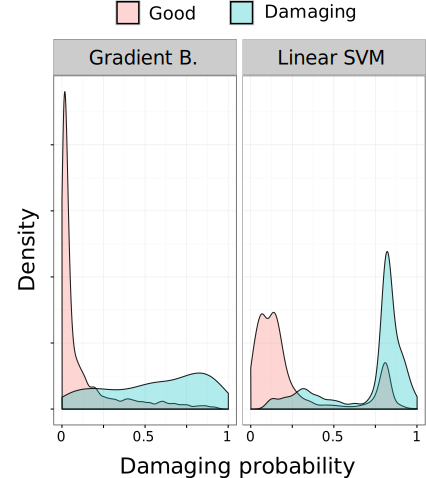
\includegraphics[width=.85\textwidth]{figures/natural_damaging_gb_vs_svc}
  \caption{No injected features}
  \label{fig:natural_damaging_gb_bs_svc}
\end{subfigure}~~
\begin{subfigure}[t]{.33\textwidth}
  \centering
  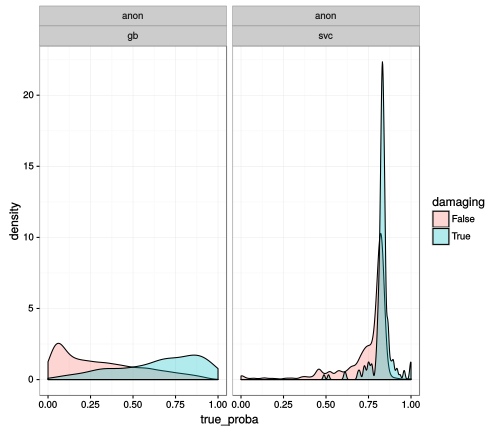
\includegraphics[width=.85\textwidth]{figures/anon_damaging_gb_vs_svc}
  \caption{Everyone is anonymous}
  \label{fig:anon_damaging_gb_bs_svc}
\end{subfigure}~~
\begin{subfigure}[t]{.33\textwidth}
  \centering
  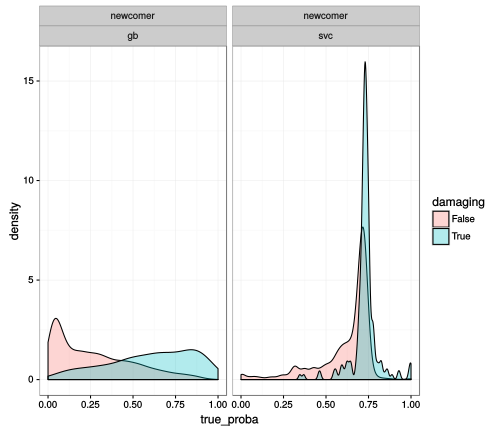
\includegraphics[width=.85\textwidth]{figures/newcomer_damaging_gb_vs_svc}
  \caption{Everyone is newly registered}
  \label{fig:newcomer_damaging_gb_bs_svc}
\end{subfigure}
\caption{The distributions of the probability of a single edit being scored as ``damaging'' based on injected features for the target user-class is presented.  Note that when injecting user-class features (anon, newcomer), all other features are held constant.}
\label{fig:prediction_error_for_anons_and_newcomers}
\end{figure*}


Figure~\ref{fig:prediction_error_for_anons_and_newcomers} shows the probability density of the likelihood of ``damaging'' given three different passes over the exact same test set, using two of our modeling strategies.  Figure~\ref{fig:natural_damaging_gb_bs_svc} shows that, when we leave the features to their natural values, it appears that both models are able to differentiate effectively between damaging edits (high-damaging probability) and non-damaging edits (low-damaging probability) with the odd exception of a large amount of non-damaging edits with a relatively high-damaging probability around 0.8 in the case of the Linear SVM model.  Figures~\ref{fig:anon_damaging_gb_bs_svc} and \ref{fig:newcomer_damaging_gb_bs_svc} show a stark difference.  For the scores that go into these plots, characteristics of anonymous editors and newly registered editors were injected for all of the test edits.  We can see that the GradientBoosting model can still differentiate damage from non-damage while the Linear SVM model flags nearly all edits as damage in both case.

Through the reporting of this issue and our subsequent analysis, we were able to identify the issue and show that an improvement to our modeling strategy mitigates the problem.  Without such a tight feedback loop, we most likely would not have noticed how poorly ORES's damage detection models were performing in practice.  Worse, it might have caused vandal fighters to be increasingly (and inappropriately) skeptical of contributions by anonymous editors and newly registered editors---two groups of contributors that are already met with unnecessary hostility\footnote{\url{http://enwp.org/:en:Wikipedia:IPs_are_human_too}}\cite{halfaker2013rise}.

\subsection{Discussion}
These case studies in responses to ORES provide a window into how our team has been able to work with editors, developers, and other stakeholders in various wiki communities around machine learning. ORES as a socio-technical system has helped us 1) refine our understandings of volunteers' needs across wiki communities, 2) identify and adress biases in ORES's models, and 3) reflect on how people think about what types of automation they find acceptable in their \emph{spaces}.

\leadin{Refining our understandings and iterating our models}
The information divide between us researchers/engineers and the members of a community (or users of a platform) is often wider than we realize.  Through iteration with the Wikidata and Italian models, we learned about incorrect assumptions we would made about how edits take place (e.g. client edits in Wikidata) and how language works (e.g. ``ha'' does not signify laugher in Italian).  It is quite likely we would never be able to fully understand the context in which damage detection models should operate before deploying the models.  Yet with a tight communication loop, many surprising and wrong assumptions that were baked into our modeling process could be identified and addressed quickly.  It seems that many of the relevant issues in feature engineering and model tuning become apparent when the model is used in context to try to address a real problem (in these cases, counter-vandalism).

\leadin{Methods for recognizing and addressing bias}
The Italian Wikipedians showed us something surprising and interesting about collaborative evaluation of machine prediction: thematic analysis is very powerful.  Through the collection of ORES mistakes and iteration, our Italian collaborators helped us understand general trends in the types of mistakes that ORES made.  It strikes us that this a somewhat general strategy for bias detection.  While our users certainly brought their own biases to their audit of ORES, they were quick to discover and come to consensus about trends in ORES's issues.  Before they had performed this process and shared their results with us, we had no idea that any issues were present. When we applied the kinds of standard fitness metrics that are expected in academic machine learning research, the damage detection model looked good enough to publish.  Their use of thematic analysis is powerful tool that developers should investigate and potentially support through new user interfaces when creating any crowd-based auditing support technologies.

\leadin{How people think about ``acceptable'' automation}
Our third case shows how ORES made possible a potentially problematic bot, but also supports Spanish Wikipedians in the process of coming to agreements about what roles are acceptable for automated agents.  Through observation of PatruBOT's behavior, they have decided that the \emph{false discovery rate} (i.e., $1 - \text{precision}$) was too high by watching the bot work in practice and they started their own independent analysis to find quantitative answers about what the ideal rate is.  Eventually they may come to a conclusion about an acceptable \emph{false discovery rate}, or they may decide that no revert is acceptable without human intervention.
